
\SbSSCT{Environnement Scope}{Environment Scope}

\begin{center}
\RRR{12-3}
\end{center}

\begin{tabular}{|c|c|} \hline
\parbox[b]{8cm}{
\BS{begin}\AC{tikzpicture}[line width = 3mm] \\ \\
\BS{draw}  (0.5,6) - - (2.5,6);\\

\ESS{scope}[{\color{red}red}] \\
\BS{draw} (0.5,5) - - (2.5,5); \\
\BS{draw}  (0.5,4) - - (2.5,4);\\
\BS{end\AC{scope}} \\ \\
\BS{draw}  (0.5,3) - - (2.5,3);\\ \\
\ESS{scope}[{\color{red}green}] \\
\BS{draw}  (0.5,2) - - (2.5,2);\\
\BS{draw} [{\color{red}red}] (0.5,1) - - (2.5,1);\\
\BS{draw}  (0.5,0) - - (2.5,0);\\
\BS{end\AC{scope}} \\ \\
\BS{end}\AC{tikzpicture}
}
&  
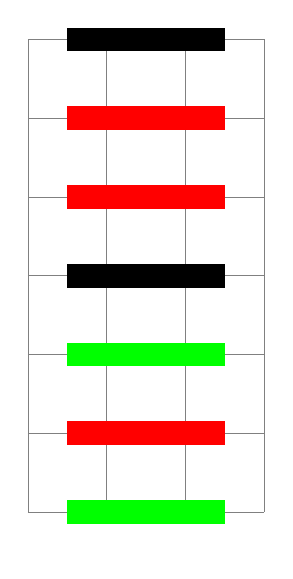
\begin{tikzpicture}[line width = 3mm,baseline=-.5cm]
\draw[help lines] (0,0) grid (3,6);
\draw (0.5,6) -- (2.5,6);
\begin{scope}[red]
\draw (0.5,5) -- (2.5,5);
\draw (0.5,4) -- (2.5,4);
\end{scope}
\draw (0.5,3) -- (2.5,3);
\begin{scope}[green]
\draw (0.5,2) -- (2.5,2);
\draw[red]  (0.5,1) -- (2.5,1);
\draw (0.5,0) -- (2.5,0);
\end{scope}
\end{tikzpicture}
\\ \hline 
\end{tabular} 

\subsection{library scopes} 

\SbSbSSCT{Simplification d'un environnement scope}{Shorthand for Scope Environments}

\begin{center}
\RRR{12-3-2}
\end{center}

 \maboite{\BS{usetikzlibrary}\AC{scopes}}
\label{lib-scopes}

\begin{tabular}{|c|c|} \hline
\parbox[b]{8cm}{
\BS{begin}\AC{tikzpicture}[line width = 3mm] \\ \\
\BS{draw}  (0.5,6) - - (2.5,6);\\ \\
{\color{red} \{} [red] \\
\BS{draw} (0.5,5) - - (2.5,5); \\
\BS{draw}  (0.5,4) - - (2.5,4);\\
{\color{red} \} } \\ \\
\BS{draw}  (0.5,3) - - (2.5,3);\\ \\
{\color{red} \{ }[green] \\
\BS{draw}  (0.5,2) - - (2.5,2);\\
\BS{draw} [{\color{red}red}] (0.5,1) - - (2.5,1);\\
\BS{draw}  (0.5,0) - - (2.5,0);\\
{\color{red} \} }\\ \\
\BS{end}\AC{tikzpicture}
}
&  
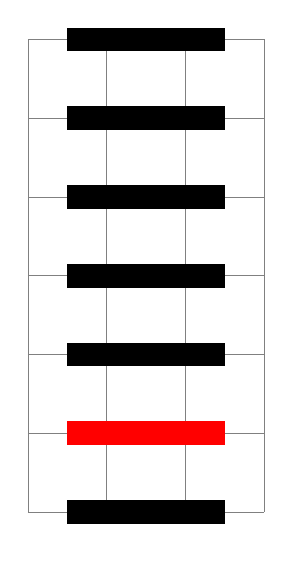
\begin{tikzpicture}[line width = 3mm,baseline=-.5cm]
\draw[help lines] (0,0) grid (3,6);
\draw (0.5,6) -- (2.5,6);
{[red]
\draw (0.5,5) -- (2.5,5);
\draw (0.5,4) -- (2.5,4);
}
\draw (0.5,3) -- (2.5,3);
{[green]
\draw (0.5,2) -- (2.5,2);
\draw [red] (0.5,1) -- (2.5,1);
\draw (0.5,0) -- (2.5,0);
}
\end{tikzpicture}
\\ \hline 
\end{tabular} 

\SbSbSSCT{Portée d'un seul élément} {Single Command Scopes}

\begin{tabular}{|c|c|} \hline
\begin{tikzpicture}
\node [fill=white] at (1,1) {\DFR};
\scoped [on background layer]
\draw (0,0) grid (3,2);
\end{tikzpicture}
&
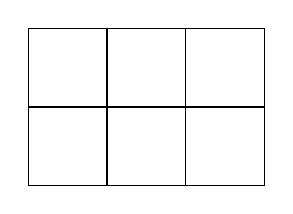
\begin{tikzpicture}
\node [fill=white] at (1,1) {\DFR};
\draw (0,0) grid (3,2);
\end{tikzpicture}
\\ \hline 
\BS{node} [fill=white] at (1,1) \AC{\BS{DFR}};  &\BS{node} [fill=white] at (1,1) \AC{\BS{DFR}}; \\
\BSS{scoped} [on background layer] & \\
\BS{draw} (0,0) grid (3,2); &  \BS{draw} (0,0) grid (3,2);
\\ \hline  
\end{tabular}